\documentclass[border=6pt]{standalone}
\usepackage{tikz}
\usetikzlibrary{arrows.meta}
\begin{document}
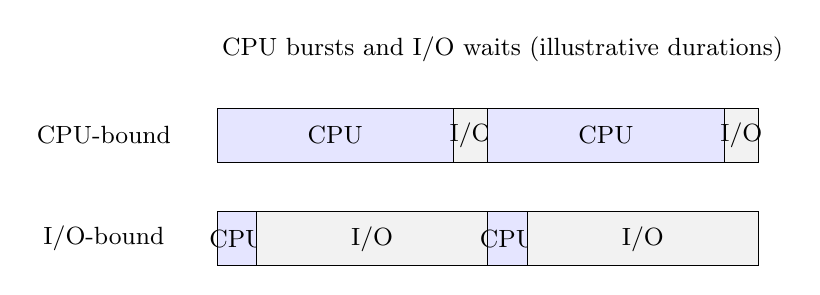
\begin{tikzpicture}[>=Stealth]
\node[align=center,font=\small] at (6.375,3.312) {CPU bursts and I/O waits (illustrative durations)};
\node[align=center,font=\small] at (1.312,2.225) {CPU-bound};
\draw[fill=blue!10] (2.750,2.562) rectangle (5.750,1.875);
\node[align=center,font=\small] at (4.250,2.219) {CPU};
\draw[fill=gray!10] (5.750,2.562) rectangle (6.188,1.875);
\node[align=center,font=\small] at (5.969,2.219) {I/O};
\draw[fill=blue!10] (6.188,2.562) rectangle (9.188,1.875);
\node[align=center,font=\small] at (7.688,2.219) {CPU};
\draw[fill=gray!10] (9.188,2.562) rectangle (9.625,1.875);
\node[align=center,font=\small] at (9.406,2.219) {I/O};
\node[align=center,font=\small] at (1.312,0.912) {I/O-bound};
\draw[fill=blue!10] (2.750,1.250) rectangle (3.250,0.562);
\node[align=center,font=\small] at (3.000,0.906) {CPU};
\draw[fill=gray!10] (3.250,1.250) rectangle (6.188,0.562);
\node[align=center,font=\small] at (4.719,0.906) {I/O};
\draw[fill=blue!10] (6.188,1.250) rectangle (6.688,0.562);
\node[align=center,font=\small] at (6.438,0.906) {CPU};
\draw[fill=gray!10] (6.688,1.250) rectangle (9.625,0.562);
\node[align=center,font=\small] at (8.156,0.906) {I/O};
\end{tikzpicture}
\end{document}
